\chapter{Fonctionnement et Tests}

Dans cette partie nous allons tout d'abord nous pencher sur le fonctionnement et les tests concernant la partie parser du projet, puis nous aborderons les mêmes points pour la partie analyse des données.

\section{Parser}

Cette partie du projet est écrite en Java. Nous avons utilisé \textit{JUnit} afin de mener à bien ces tests unitaires. De plus, le dépôt \textit{GIT} est muni d'un outil d'intégration continu (\textit{Travis}), qui garantit l'intégrité du code préexistant.\\

De plus, nous avons effectué des tests de couverture en utilisant le plugin \textit{Cobertura Maven} qui nous a aidé à détecter les points plus faibles au niveau des tests et donc à proposer d'autres tests unitaires pour avoir une meilleure couverture.


\subsection{Politique de tests}

Le but de nos test est de verifier l'extraction des donnéees des \textit{Logs}. Pour ce faire, nous avons choisi deux \textit{Logs} réels représentatifs de chaque version et avons appliqué la stratégie suivante:  \\
\begin{itemize}
\item En premier lieu; nous avons réalisé des tests pour vérifier la bonne détection de version en présence de laquelle on se trouve.
\item Ensuite, nous avons pris chaque donnée de la structure et avons validé qu'elle ne soit pas vide. Dans le cas où l'élément est une liste, nous vérifions que le nombre d'éléments de la liste correspond au nombre d'éléments dans le \textit{Log}, 
\item Et finalement, pour les éléments carte/quantité, comme par exemple \textit{Victory Cards} ou \textit{Market} nous vérifions que le couple (nom, valeur) correspond.
\end{itemize}


\subsection{Tests unitaires}

Les tests proposés pour la validation du module Java sont fait avec des \textit{Logs} réels et sans aucune altération.\\
Nous avons utilisé six \textit{Logs}, deux représentatifs de chaque type de version de \textit{Logs} (3 versions actuellement). \\

Dans la classe \textit{LogReaderFactoryTest}, nous voulons tester la lecture du \textit{Log}, la création de l'objet \textit{LogReader} qui instancie la version correspondante du parser et la construction de l'objet \textit{Document} complet avec toutes les données du \textit{Log} à envoyer à la base de données. \\

Dans les classes \textit{LogReaderV1HeaderTest}, \textit{LogReaderV2HeaderTest }et \textit{LogReaderV3HeaderTest}, on rentre dans le détail de l'objet Document, et on vérifie que les attributs Date, Name, Winners, Cards Gone, Cards Market et Cards Trash sont corrects au niveau des noms, nombre et quantité par rapport aux informations contenues dans les \textit{Logs}. \\

Dans la classe \textit{LogReaderPlayerTest}, on valide les données propres du joueur. Pour les tests, on utilise trois \textit{Logs}, un pour chaque version de parser et pendant les test, on prend un joueur au hasard pour chaque \textit{Log}. On verifie que le nombre de joueurs correspond ou nombre de joueurs du \textit{Log}. Les noms des joueurs doivent correspondre au nom des joueurs du \textit{Log}. Le même principe est appliqué pour les points et le nombre de tours. \\
Pour les données de \textit{Cards Victory}, \textit{Cards Deck}, \textit{Cards FirstHand} et \textit{Cards Opening}, on valide le nombre, le nom et la quantite par rapport aux \textit{Logs}. \\

Finalement, on teste la classe \textit{PlayerTest} afin qu'il n'y ait pas de duplications de joueurs.

\begin{figure}[!h]
  \begin{center}
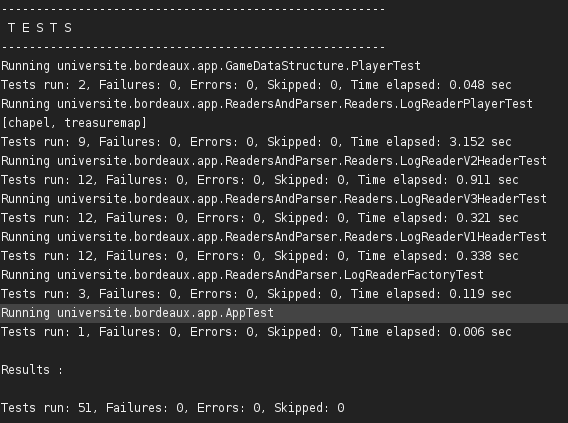
\includegraphics[width=\textwidth,height=\textheight,keepaspectratio]{./unit_tests_jave}
  \end{center}
  \caption{Résultats des tests unitaires pour le parser}
\end{figure}

Avec un total de 51 test executés, aucune erreur ou aucun échec n'ont été détectés.

\subsection{Tests de couverture}
Voici les resultats obtenus lors des tests de couverture de la partie Parser du projet:

\begin{figure}[!h]
  \begin{center}
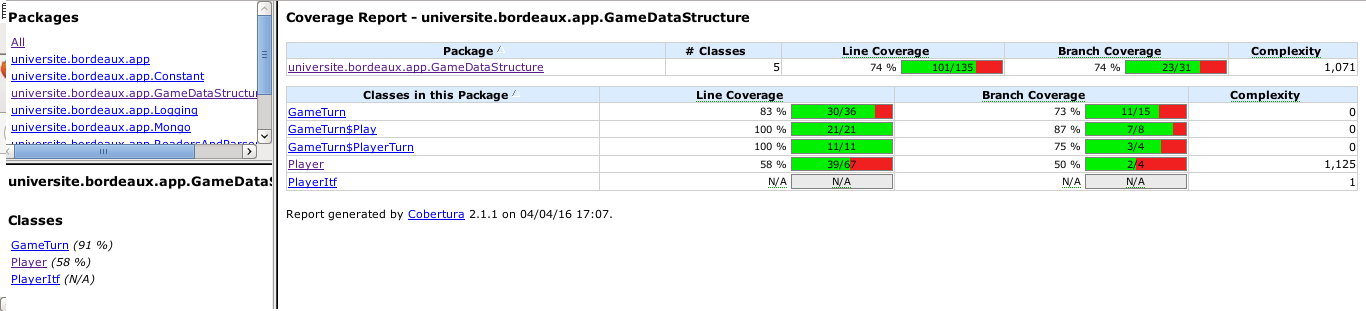
\includegraphics[width=\textwidth,height=\textheight,keepaspectratio]{./coverage_GameDataStructure}
\end{center}
  \caption{Résultats des tests de couverture pour la structure de données}
  \end{figure}

Dans la partie structure de données, nous n'avons pas testé l'utilisation d'actions successives dans un même tour (combo). L'autre portion de code non testée correspond à la conversion des données d'un joueur contenues dans le serveur vers un objet de type \textit{Player}. Ce cas de figure ne se produit jamais avec l'utilisation envisagée pour la partie Java. Mais si jamais le projet venait à évoluer et utiliser des données de joueurs déja présentes dans le serveur, il faudrait effectuer des tests sur cette partie.

\begin{figure}[!h]
  \begin{center}
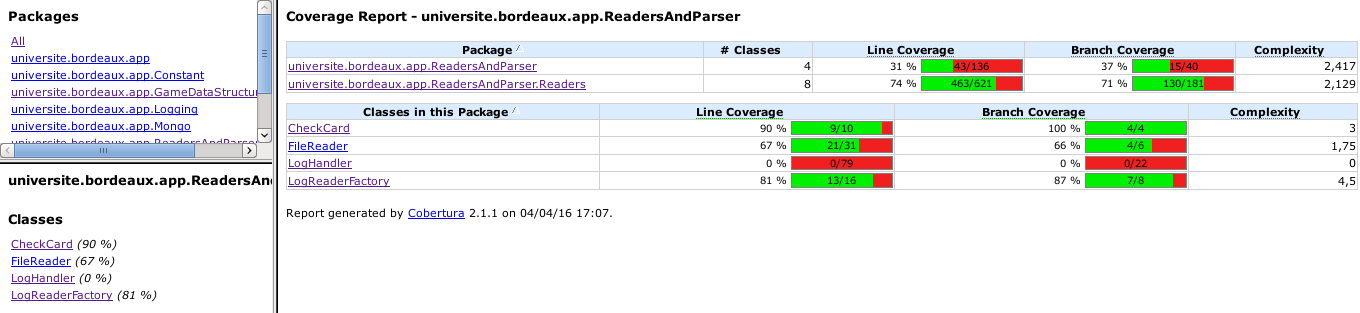
\includegraphics[width=\textwidth,height=\textheight,keepaspectratio]{./coverage_ReadersAndParser}
\end{center}
  \caption{Résultats des tests de couverture pour la création des différent parsers}
\end{figure}

Pour la partie préparant le parsing (c'est-à-dire avant l'utilisation du parser), par manque de temps, nous n'avons pas pu tester le \textit{LogHandler}. Pour le module \textit{FileReader}, nous n'avons pas testé les cas aux limites, ce qui entraine la non-couverture des lancement d'exceptions. Pour le module \textit{LogReaderFactory}, la portion non traitée correspond au cas où une partie du header d'un \textit{Log} est manquante. Il aurait fallu rajouter un test pour ce cas de figure.

\begin{figure}[!h]
  \begin{center}
    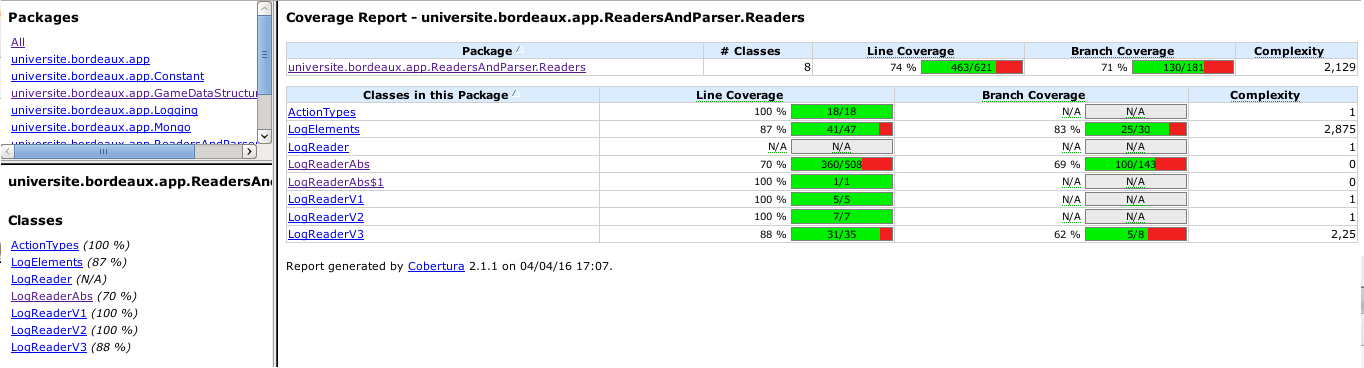
\includegraphics[width=\textwidth,height=\textheight,keepaspectratio]{./coverage_ReadersLog}
  \end{center}
  \caption{Résultats des tests de couverture pour les différentes versions de parsers}
\end{figure}

Pour le module \textit{LogReaderAbs}, nous n'avons pas testé le cas de figure où plusieurs joueurs gagnent en étant ex-aequo. Le reste du code non couvert correspond à des cas de figures plus rares. Pour obtenir une couverture de ces portions de code, il aurait fallu trouver ou bien construire des \textit{Logs} plus variés. Un certain nombre de facteurs, dont le temps nous a empêché d'effectuer ce travail assez long.

\subsection{Bugs rencontrés}

\paragraph*{Dictionnaire de Cartes} 

Il existe une classe qui sert à verifier l'existence d'une carte et redonner en même temps le nom générique de la carte donnée.\\
Il y a des problèmes avec les cartes dont le pluriel change radicalement du singulier, par exemple les cartes Colonies (Colony) et Duchies (Duchy). \\

Pour résoudre le bug il faut changer le dictionaire actuellemement implementé, pour ajouter la conversion de cartes dont le nom au pluriel est plus compliqué que le simple ajout d'un "s".


Pour la classe \textit{LogReaderAbs}, il y a des actions qui ne sont pas testées car, dans les \textit{Logs} selectionnés pour les tests, il n'existe pas toutes les actions possibles pour les joueurs, Une solution serait d'augmenter la sélection des \textit{Logs} utilisés, pour disposer d'une gamme plus significative d'exemples.


\section{Module d'analyse des donnée}
Cette partie du projet écrite en Python est cruciale, car c'est elle qui sera mise à disposition de  l'utilisateur. Nous avons utilisé le module \textit{pytest} pour effectuer nos tests unitaires ainsi que \textit{mongomock} pour simuler l'utilisation d'un serveur \textit{MongoDB}. Les tests de couverture ont été effectués à l'aide de \textit{pytest-cov}.

\subsection{Politique de tests}
La stratégie choisie pour les tests a été de les effectuer après le développement. Nouys avons utilisé les outils suivants : 
\begin{itemize}
\item \textit{Pytest}, un framework destiné à faciliter la création de petits tests, efficaces même pour des fonctions complexes.
\item \textit{Mongomock}, petite bibliothèque destinée à aider au test de code Python en interaction avec MongoDB.
\item un fichier Python sur lequel on crée un dictionnaire représentant un document dans la base de données (\textit{Logtest}).
\end{itemize}

\subsection{Tests unitaires}
\paragraph{module Match}
Trois tests unitaires ont été effectués:
\begin{itemize}
\item un test de comparaison du nom des joueurs.
\item un test de comparaison des \textit{Logs} à proprement parler par rapport à un \textit{Log} standard, c'est à dire la vérification que les actions des joueurs au cours de la partie sont bien chargées dans la structure de données. 
\item un test de comparaison des informations du \textit{header} par le même procédé.
\end{itemize}

Ces trois tests passent sans poser de problèmes.

\paragraph{Module Tools}
Trois tests unitaires ont été effectués:
\begin{itemize}
\item un premier test permet de vérifier la bonne création de la pseudo base de données (utilisation de \textit{mongomock}).
\item un second test vérifie la bonne création des informations globales pour chaque joueur présent dans le log test (2 joueurs).
\item le troisième test vérifie que la fonction de calcul d'ELO s'applique correctement, de même que la détection du \textit{greening}.
\end{itemize}

\subsection{Tests de couverture}
Le résultat des tests de couverture est le suivant:

\begin{figure}
  \begin{center}
    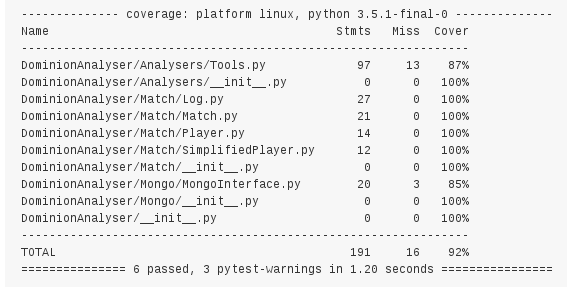
\includegraphics[width=\textwidth,height=\textheight,keepaspectratio]{./coverage_python_code}
  \end{center}
  \caption{Résultat des tests de couverture concernant la partie Analyse des données}
\end{figure}

Nous ne couvrons pas totalement le module \textit{Tools} ; cela s'explique par le fait que nous n'avons pas fait de tests sur la reconaissance des stratégies.\\
Le module \textit{MongoInterface} n'est pas entièrement couvert non plus, car nous ne testons pas la création d'index et de collections.


\paragraph{Conclusions}

Nous n'avons pas pu effectuer plus de tests mais une suite logique à ces quelques tests unitaires serait de produire des \textit{Logs} pouvant poser problème, par exemple avec des caractères spéciaux ou bien des mots clefs relatifs au langage Python. Concernant les test unitaires des outils, d'autres tests pourraient être effectués pour la detection des stratégies ou bien pour des valeurs d'ELO ambigües.


%La partie programmation a demandé beaucoup de travail et a été quasiment le fait d’un seul membre du projet, qui ne pouvait également réaliser la partie test. La répartition du travail ayant abouti à confier les tests aux autres membres de l’équipe, la faible quantité de tests réalisée ne fait que traduire une implication trop limitée et très tardive de ceux-là.
